% ============================================================================
%  BLOQUE V — DIAPOSITIVAS 18–21: INTEGRACIÓN DE HARDWARE
% ============================================================================
\section{Integración de Hardware}

% ----------------------------------------------------------------------------
%  DIAPOSITIVA 18 — TUYA + HOTSPOT SPOOFING
% ----------------------------------------------------------------------------
\begin{frame}{5 — Integración Tuya: Control Local y Hotspot Spoofing}
  \hypertarget{s:tuya}{}

  \IfFileExists{figures/19_tuya.pdf}{%
    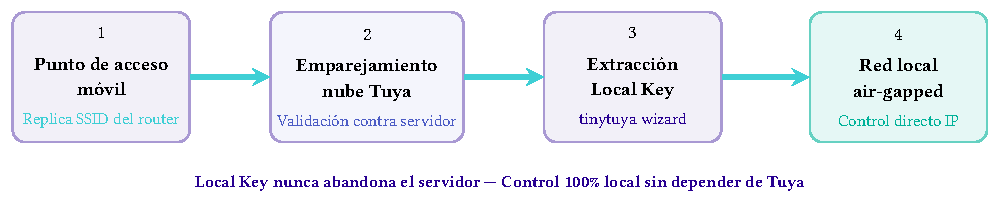
\includegraphics[width=\textwidth, height=4.2cm, keepaspectratio]{figures/19_tuya.pdf}%
  }{
    \textcolor{darkgray}{[Figura: 4 pasos Hotspot Spoofing]}
  }

  \vspace{0.3cm}
  \begin{columns}[T]
    \column{0.35\textwidth}
    \IfFileExists{\memoriaimg/hw_tuya_plug.png}{%
      
\includegraphics[height=3cm, keepaspectratio]{\memoriaimg/hw_tuya_plug.png}%
    }{
      \fbox{\parbox{0.8\textwidth}{\centering\footnotesize [Enchufe Tuya]}}
    }

    \column{0.65\textwidth}
    \footnotesize
    \textbf{Protocolo \texttt{tinytuya} 3.5}\\
    Local Key en servidor · Respuesta $<$2 s\\
    Control ON/OFF validado en red air-gapped
  \end{columns}
\end{frame}

% ----------------------------------------------------------------------------
%  DIAPOSITIVA 19 — BLE XIAOMI GATT
% ----------------------------------------------------------------------------
\begin{frame}{5 — Sensores BLE Xiaomi: Lectura GATT Directa}
  \hypertarget{s:xiaomi}{}
  \begin{columns}[T]
    \column{0.58\textwidth}
    \centering
    \IfFileExists{\memoriaimg/fig_8_5.pdf}{%
      
\includegraphics[width=\textwidth, height=5.5cm, keepaspectratio]{\memoriaimg/fig_8_5.pdf}%
    }{%
      \fbox{\parbox{0.9\textwidth}{\centering\footnotesize [Decodificación BLE]}}
    }

    \column{0.42\textwidth}
    \centering
    \IfFileExists{\memoriaimg/hw_xiaomi_sensor.png}{%
      
\includegraphics[height=3.5cm, keepaspectratio]{\memoriaimg/hw_xiaomi_sensor.png}%
    }{
      \fbox{\parbox{0.6\textwidth}{\centering\tiny [Sensor]}}
    }\\[0.1cm]
    {\footnotesize Xiaomi LYWSD03MMC}

    \vspace{0.1cm}
    \begin{exampleblock}{Lectura GATT directa}
      \footnotesize
      Decodificación de temperatura, humedad y batería\\
      directamente del sensor, sin \textit{bind key} · Sin nube Xiaomi
    \end{exampleblock}
  \end{columns}
\end{frame}

% ----------------------------------------------------------------------------
%  DIAPOSITIVA 20 — FANLAMP: INGENIERÍA INVERSA
% ----------------------------------------------------------------------------
\begin{frame}{5 — FanLamp F8808: Ingeniería Inversa del Protocolo}
  \hypertarget{s:fanlamp}{}

  \centering
  \IfFileExists{figures/21_fanlamp.pdf}{%
    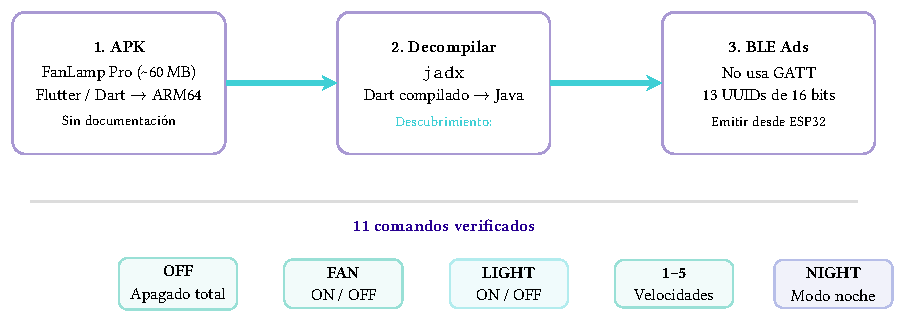
\includegraphics[width=\textwidth, height=3.8cm, keepaspectratio]{figures/21_fanlamp.pdf}%
  }{
    \textcolor{darkgray}{[Figura: ingeniería inversa FanLamp]}
  }

  \vspace{0.2cm}
  \begin{columns}[T]
    \column{0.35\textwidth}
    \IfFileExists{\memoriaimg/hw_fanlamp.png}{%
      
\includegraphics[height=2.8cm, keepaspectratio]{\memoriaimg/hw_fanlamp.png}%
    }{
      \fbox{\parbox{0.8\textwidth}{\centering\footnotesize [FanLamp F8808]}}
    }\\[0.05cm]
    {\footnotesize Mikomika F8808 — 35 € AliExpress}

    \column{0.65\textwidth}
    \footnotesize
    \begin{exampleblock}{Descubrimiento clave}
      APK FanLamp Pro decompilado (\texttt{jadx})\\
      \alert{No usa GATT, sino anuncios BLE}\\
      11 comandos mapeados — emitidos desde ESP32 vía USB
    \end{exampleblock}
  \end{columns}
  \vspace*{-0.2pt}
\end{frame}
